\section{Evaluation: Distributed Matrix-Vector Multiplication}
\label{sec:evaluation}

To validate the latency model of Section~\ref{sec:switching} and to demonstrate
HyNoC in a concrete distributed computing scenario, we implemented a
Verilator~\cite{verilator}-based simulation of a $4\times4$ mesh executing a
distributed matrix-vector multiplication.  The benchmark covers the full
communication cycle: data scatter from a master, computation at worker nodes, and
result gather back to the master.

\subsection{Network Topology}

The network consists of 16~\texttt{hynoc\_router\_5p} instances arranged as
a $4\times4$ 2D mesh, as shown in Figure~\ref{fig:mesh4x4}.  Routers are
addressed by $(r,c)$ with $r\in\{0,1,2,3\}$ (row, top-to-bottom) and
$c\in\{0,1,2,3\}$ (column, left-to-right).  Port convention per router:
0\,=\,Local, 1\,=\,East, 2\,=\,South, 3\,=\,West, 4\,=\,North.  Each
router's local port (port~0) attaches a processing node; neighboring routers are
cross-linked on their directional ports (e.g., router $(r,c)$ port~1 connects to
router $(r,c{+}1)$ port~3).

\begin{figure}[t]
  \centering
  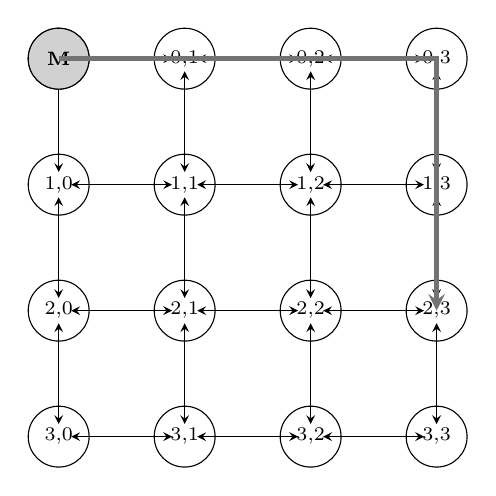
\begin{tikzpicture}[
    rtr/.style={circle, draw, font=\scriptsize, inner sep=1pt, minimum size=22pt},
    mst/.style={circle, draw, fill=black!18, font=\scriptsize\bfseries, inner sep=1pt,
                minimum size=22pt},
    >=stealth,
    route/.style={->, line width=1.6pt, color=black!55}
  ]
  \def\S{1.6}
  % Horizontal links
  \foreach \row in {0,...,3}{
    \foreach \col in {0,...,2}{
      \draw[<->] ({\col*\S+0.16},{-\row*\S}) -- ({\col*\S+\S-0.16},{-\row*\S});
    }
  }
  % Vertical links
  \foreach \row in {0,...,2}{
    \foreach \col in {0,...,3}{
      \draw[<->] ({\col*\S},{-\row*\S-0.16}) -- ({\col*\S},{-\row*\S-\S+0.16});
    }
  }
  % All nodes
  \foreach \row in {0,...,3}{
    \foreach \col in {0,...,3}{
      \node[rtr] at ({\col*\S},{-\row*\S}) {\row,\col};
    }
  }
  % Master override
  \node[mst] at (0,0) {\textbf{M}};
  % Sample route (0,0)→(2,3): East×3, South×2
  \draw[route] (0,0) -- ({\S},0) -- ({2*\S},0) -- ({3*\S},0)
               -- ({3*\S},{-\S}) -- ({3*\S},{-2*\S});
  \end{tikzpicture}
  \caption{$4\times4$ mesh topology. \textbf{M} = master at $(0,0)$; remaining
           nodes are workers at $(r,c)$.  Bidirectional links are full-duplex
           (independent ingress and egress).  The gray arrow illustrates the XY
           route from the master to worker $(2,3)$: three East hops followed by two
           South hops, then a final local hop ($H=6$).}
  \label{fig:mesh4x4}
\end{figure}

The master node resides at $(0,0)$.  It sequentially distributes data to all 15
worker nodes and collects their results.

\subsection{Computation and Communication Model}

The benchmark computes $\mathbf{y} = A\mathbf{x}$ with $A\in\mathbb{R}^{16\times4}$
and $\mathbf{x}=[1,2,3,4]^T$.  Worker $(r,c)$ is responsible for one scalar inner
product: $y_{4r+c} = \langle A_{4r+c},\, \mathbf{x} \rangle$.

\textbf{Forward packet} (master to worker $(r,c)$): one routing flit, one tag
flit, four flits for the matrix row $A_{4r+c}$, and four flits for
$\mathbf{x}$, totaling ten flits.  After the routing flit is consumed by the
network, the worker receives $P_\text{fwd}=9$ payload flits.

\textbf{Return packet} (worker to master): one routing flit, one tag flit, and one
result flit.  The master receives $P_\text{ret}=2$ payload flits.

Workers compute the inner product instantaneously, so the total simulation time
is dominated by communication latency and the sequential injection schedule at
the master.

\textbf{XY routing.}  Packets follow dimension-order routing: East/West moves
bring the packet to the target column, North/South moves bring it to the target
row, and a final local hop delivers it.  This eliminates cyclic channel
dependencies and guarantees deadlock freedom~\cite{dally1987}.  A route from
$(r_0,c_0)$ to $(r_1,c_1)$ requires
\begin{equation}
  H = |c_1-c_0| + |r_1-r_0| + 1
  \label{eq:hops-xy}
\end{equation}
hops, including the final local hop.  For the master at $(0,0)$, this simplifies
to $H=r+c+1$.  Routes are encoded as source-routing flits using the relative hop
encoding described in Section~\ref{sec:architecture}.

\subsection{Simulation Infrastructure}

The Verilator C++ model instantiates 16~\texttt{Vhynoc\_router\_5p} objects
sharing one \texttt{VerilatedContext}.  Inter-router links are modeled as
one-cycle latches: egress signals are captured after each rising clock edge and
applied to the neighbor's ingress before the next rising edge.  This one-cycle
propagation delay is physically accurate for a registered synchronous
interconnect.

Each router drives a single clock (\texttt{router\_clk} and all
\texttt{portX\_ingress\_clk} toggled together).  In dual-clock mode
(\texttt{SINGLE\_CLOCK\_ROUTER=0}), the ingress dual-clock FIFOs internally
use gray-code CDC synchronization even when source and destination clocks are
the same signal; in single-clock mode (\texttt{SINGLE\_CLOCK\_ROUTER=1}), the
gray-code pipeline is bypassed.

\subsection{Latency Results}

Table~\ref{tab:latency} reports the \emph{return-path} latency for each hop
count $H$ in both configurations.  Return-path measurements are free of
source-queuing effects (each worker sends exactly one result as soon as
computation completes), yielding clean linear fits.

\begin{table}[h]
\centering
\footnotesize
\setlength{\tabcolsep}{4pt}
\caption{Return-path latency ($P=2$) vs.\ hop count}
\label{tab:latency}
\begin{tabular}{@{}rrrrrr@{}}
\toprule
 & \multicolumn{2}{c}{Simulated (cy.)} & & \multicolumn{2}{c}{Theory~(\ref{eq:latency})} \\
\cmidrule(lr){2-3}\cmidrule(lr){5-6}
$H$ & Dual & Single & $\Delta$ & Dual & Single \\
\midrule
2 & 25 & 19 &  6 & 13 &  9 \\
3 & 37 & 28 &  9 & 19 & 13 \\
4 & 49 & 37 & 12 & 25 & 17 \\
5 & 61 & 46 & 15 & 31 & 21 \\
6 & 73 & 55 & 18 & 37 & 25 \\
7 & 85 & 64 & 21 & 43 & 29 \\
\bottomrule
\end{tabular}
\end{table}

The measured latencies satisfy exact linear fits:
\begin{align}
  L_\text{dual}   &= 12H + P - 1 \label{eq:lfit-dual}   \\
  L_\text{single} &= 9H + P - 1  \label{eq:lfit-single}
\end{align}
Both fits are consistent with the model of~(\ref{eq:latency}): latency scales
linearly with hop count, with a per-hop coefficient determined by
$T_\text{FIFO}$, the FSM decode cycle, and $T_\text{PRRA}$.
The theoretical minimum slopes (PIPELINE=0) are $6H$ for dual-clock
($T_\text{FIFO}\approx3$) and $4H$ for single-clock ($T_\text{FIFO}=1$).
The simulation slopes are higher for two reasons: (i) the gray-code
synchronization pipeline incurs additional latency when source and destination
clocks are the same signal, as is the case in this single-clock Verilator
environment; and (ii) the one-cycle inter-router link latch adds one cycle per
hop.  Both effects vanish in a real FPGA deployment where clock domains differ
and wiring is combinatorial within the same clock cycle.

The critical result is the \textbf{improvement margin}: theory predicts a
difference of $2H$ cycles between the two modes; simulation measures $3H$,
the extra cycle per hop being exactly the CDC overhead eliminated by
single-clock operation.  The reduction is constant and perfectly linear,
confirming the deterministic nature of the HyNoC latency model.

The total simulation time is \textbf{391~cycles} in dual-clock mode and
\textbf{349~cycles} in single-clock mode ($-$10.7\%).  All 16 computed
results are correct in both runs.

\subsection{Link Utilization}

Table~\ref{tab:links} summarizes link utilization over the 391-cycle dual-clock run.
Traffic is inherently asymmetric: the master sends all forward packets via its East
port first, concentrating load on the East-bound links of row~0.

\begin{table}[h]
\centering
\footnotesize
\setlength{\tabcolsep}{4pt}
\caption{Link utilization (\%) by direction (dual-clock, 391 cycles).
         Seg.\,k: $k$-th link from master $(0,0)$.}
\label{tab:links}
\begin{tabular}{@{}lrrr@{}}
\toprule
Direction & Seg.\,1 & Seg.\,2 & Seg.\,3 \\
\midrule
$\to$East, row\,0  & 30.7 & 20.5 & 10.2 \\
$\to$West, row\,0  &  2.3 &  1.5 &  0.8 \\
$\to$South, col\,0 &  7.7 &  5.1 &  2.6 \\
$\to$North, col\,0 &  9.2 & \multicolumn{2}{c@{}}{---} \\
\midrule
\multicolumn{4}{@{}l}{\textbf{Overall average: 3.3\%}} \\
\bottomrule
\end{tabular}
\end{table}

East-bound utilization halves at each column of row~0, consistent with XY
routing: each router delivers one packet to its local worker and forwards the
rest eastward.  The overall average of 3.3\% reflects the sequential master
bottleneck: with a single sender issuing one packet at a time, most links are
idle.  In a multi-master or pipelined injection scenario, utilization scales
proportionally with the number of concurrent senders, and the rich path
diversity of the mesh (20 shortest paths between corner nodes,
Table~\ref{tab:paths}) provides ample room for congestion distribution.
